\documentclass[conference]{IEEEtran}
\IEEEoverridecommandlockouts
% The preceding line is only needed to identify funding in the first footnote. If that is unneeded, please comment it out.
\usepackage{cite}
\usepackage{amsmath,amssymb,amsfonts}
\usepackage{algorithmic}
\usepackage{graphicx}
\usepackage{textcomp}
\usepackage{xcolor}
\def\BibTeX{{\rm B\kern-.05em{\sc i\kern-.025em b}\kern-.08em
    T\kern-.1667em\lower.7ex\hbox{E}\kern-.125emX}}
\begin{document}

\title{Edge Computing Testbed for V2I Applications Prototyping and Evaluation *\\
{\footnotesize \textsuperscript{*}Note: Sub-titles are not captured in Xplore and
should not be used}
\thanks{This work is funded by Alan Turing??}
}

\author{\IEEEauthorblockN{1\textsuperscript{st} Zeinab Nezami}
\IEEEauthorblockA{\textit{School of Computing} \\
\textit{University of Leeds}\\
Leeds, United Kingdom \\
z.nezami@leeds.ac.uk}
\and
\IEEEauthorblockN{2\textsuperscript{nd} Evangelos Pournaras}
\IEEEauthorblockA{\textit{School of Computing} \\
\textit{University of Leeds}\\
Leeds, United Kingdom \\
e.pournaras@leeds.ac.uk}
\and
\IEEEauthorblockN{3\textsuperscript{th} Professor Jie Xu}
\IEEEauthorblockA{\textit{School of Computing} \\
\textit{University of Leeds}\\
Leeds, United Kingdom\\
j.xu@leeds.ac.uk}
}

\maketitle

\begin{abstract}
This paper presents ATEDGEV2I an edge computing testbed built with real devices to support the testing of V2I applications. ATEDGEV2I extends the range of end devices using mobile and migration management strategy and simple application programming interfaces (API) for testbed users. It provides access across University of Leeds campus to compute resources, and software for testing constrained vehicle to edge infrustructure applications. ATEDGEV2I runs edge workloads as sets of containers with access to specialized hardware on an expandable cluster of light-weight edge nodes which leverage institutional network to decrease implementation cost and provide wide access to resources. 
The proposed system automatically determines which edge nodes to place Docker containers on according to service requirements specified by the testbed users through APIs. Using a simple V2I application, we demonstrate that ATEDGEV2I is simple to configure.
\end{abstract}

\begin{IEEEkeywords}
Edge Computing, V2I application, Testbed, Dynamic Resource Allocation. 
\end{IEEEkeywords}

\section{Introduction}
\par Vehicle-to-infrastructure communication (V2I) is the bi-directional exchange of information between vehicles and smart road infrastructure via a wireless connection.
This technology enables vehicles to capture and transmit data such as their speed and location, traffic congestion, and bridge clearance and then transmits the information back from the infrastructure to inform the drivers of safety, mobility, or environment-related conditions. Edge computing (EC) allows for real-time data processing, which allows V2I applications and vehicles to react to data instantaneously, thereby improving safety and enhancing efficiency.
\par V2I applications should deal with various data provided through various communication links. The density and the
mobility of the vehicles are the major factors to take into account when developing V2X applications that are destined to run in mobile edge computing distributed environment. In a high-density scenario, the application must use the available resources efficiently in order to deliver its service continuously to the subscribed users. The application should also deal with nodes joining/leaving the network during their mouvement and guarantee the service continuity. 
\par An important aspect that should be taken into account while developing a V2X application that targets MEC as a deployment environment is to ensure the proper interaction of the application with the management entities and the system components. At the development phase of a V2X MEC service components testing in real environment increase deployment time, costs, and complexity. 
Experimental Testbeds have long been used to design and benchmark applications before large-scale deployments\cite{berman2014geni,ertin2006kansei,keahey2020lessons} as they are vital to gain hands-on experience with the deployment of edge-based applications and fully understand the benefits of edge computing by means of proof-of-concept demonstration. Compared with simulation and emulation, the fidelity of an overlay network built with real
equipment is the best.  
\par Designing a testbed that is extensible, easy to deploy, and useful for V2I workloads comes with challenges. 
Some of the characteristics that an edge testbed should provide\cite{boubin2022prowess} includes: 
(i) rich configurability: As many aspects of the testbed as possible should be configurable by the user, including hardware and software. (ii) Efficient resource allocation: Users should be able to request fine-grained slices of resources without encumbering their workload with unnecessary overhead. (iii) User and infrastructure security: An edge testbed should assure that data transmission, storage, and access are secure, private, and controlled.
\par To address the challenges mentioned above, we present ATEDGEV2I (Alan Turing Edge testbed for V2I applications): A scalable and open testbed architecture for general V2I applications experimentation with provisioned edge networks. ATEDGEV2I allows users to configure compute nodes quickly. It runs user code in containers, allowing users to request compute resources and execute arbitrary code without incurring the overhead of virtualization or security infrastructure of bare-metal privileged access. By attaching to secure institutional networks and sandboxing user code in containers, it maintains a secure and private testbed for user workloads. ATEDGEV2I testbed is implemented at the University of Leeds (UoL), a research-intensive Russell Group institution that contains 8 decentralized nodes provisioned on our UoL's overlay network.
\par The contributions of this work are three fold: (i) an experimental testbed for V2I application over edge computing is developed. (ii) a resource management scheme based on multi-agent systems is employed to provide guaranteed load-balancing over the edge network with respect to the resource requirements of V2I services.
(iii) support mobility by integrating testbed with the mobility tool Simulation of Urban Mobility (SUMO)\cite{behrisch2011sumo}. The testbed can be generalised to other (similar) mobility patterns also.

We build an application representing V2I workload over edge computing: real-time traffic monitoring.

\section{Related work}
\begin{table}[htbp]
\caption{Table Type Styles}
\begin{center}
\begin{tabular}{|c|c|c|c|}
\hline
\textbf{Table}&\multicolumn{3}{|c|}{\textbf{Table Column Head}} \\
\cline{2-4} 
\textbf{Head} & \textbf{\textit{Table column subhead}}& \textbf{\textit{Subhead}}& \textbf{\textit{Subhead}} \\
\hline
copy& More table copy$^{\mathrm{a}}$& &  \\
\hline
\multicolumn{4}{l}{$^{\mathrm{a}}$Sample of a Table footnote.}
\end{tabular}
\label{tab1}
\end{center}
\end{table}

...\cite{boubin2022prowess}:
Most are designed for custom workloads\cite{meng2019dedas,munoz2017adrenaline,vasisht2017farmbeats} or small user groups\footnote{Purdue Dependable Computing Systems Laboratory. 2021. Facilities and Equipment at DCSL: Testbeds. https://engineering.purdue.edu/dcsl/about/, USC Center for Cyber-Physical Systems and the Internet of Things. 2021. A
Campus-wide internet-of-Things Testbed. http://cci.usc.edu/index.php/cci-iottestbed/}, providing little or no programability, configurability and slicing.
Many testbeds have been developed for both general and specific use cases. Custom edge testbeds have been used to benchmark edge-specific algorithm and AI development\cite{hao2018edge,zhang2019hetero}, edge networking techniques\cite{meng2019dedas,munoz2017adrenaline}, offloading\cite{gedawy2016cumulus}, hardware paradigms\cite{pan2016homecloud} and diverse edge applications\cite{boubin2019managing,vasisht2017farmbeats}. Custom testbeds, however, lack the wide deployment, rich sensor availability, re-programmability, and extensibility of
major systems testbeds. Some edge testbeds, like USC’s CCI IoT Testbed [13], are wide reaching and have considerable sensor access, but lack the programmability necessary for edge experimentation.
Similarly, testbeds at Purdue University [19] are programmable, but lack the openness, orchestration, wide reach, and slicability that edge practitioners require of a general testbed...

\par Fogbed\cite{coutinho2018fogbed} propses cloud and fog testbeds that leverage mininet and docker containers. It allows  dynamically adding and removing containers
in the network topology at any time during the experiments, but it does not support the management of mobility and scalability. Cumulus\cite{gedawy2016cumulus} is a distributed edge computing testbed. It mainly centers around task offloading, and similar to Fogbed\cite{coutinho2018fogbed} do not considering the mobility of nodes.
EdgeNet\cite{cappos2018edgenet} is a kubernetes cluster that consists of a master node that manages a set of globally distributed worker nodes, i.e., deployed edge servers, running at sites across the US, Canada, and the EU. A testbed user obtains Docker containers using the Kubernetes Dashboard of EdgeNet. EdgeNet allows testbed users to select the geographical locations of servers to create Docker containers on regardless of the RTTs between the servers and wireless base station nodes.

Therefore, we modify the piFogBed\cite{xu2020support} for supporting the mobility of end devices and name it
piFogBedII. We modify piFogBed mainly from four aspects:
1. Adding mobile and migration management for end devices;
2. Expanding the range of end devices;
3. Supporting a user’s selection of fog nodes freely;
4. Inserting a container agent between internal containers and external devices to make their
interaction transparent.
\section{Testbed Design}
\par The proposed testbed aims at helping researchers and developers to design and verify
V2I applications and algorithms destined to run in an edge computing environment. ATEDGEV2I testbed is inherently a distributed system. As shown in Figure.\ref{fig:model}, it consists of at least one system orchestrator
and a set of edge nodes. Both the orchestrator and edges are separate and potentially geographically disparate pools of
compute resources connected by the institutional network. The other main components of the testbed are agent, service distributor, and connector. The following subsections outline constituent modules of ATEDGEV2I.
\begin{figure}[!htbp]
\centering
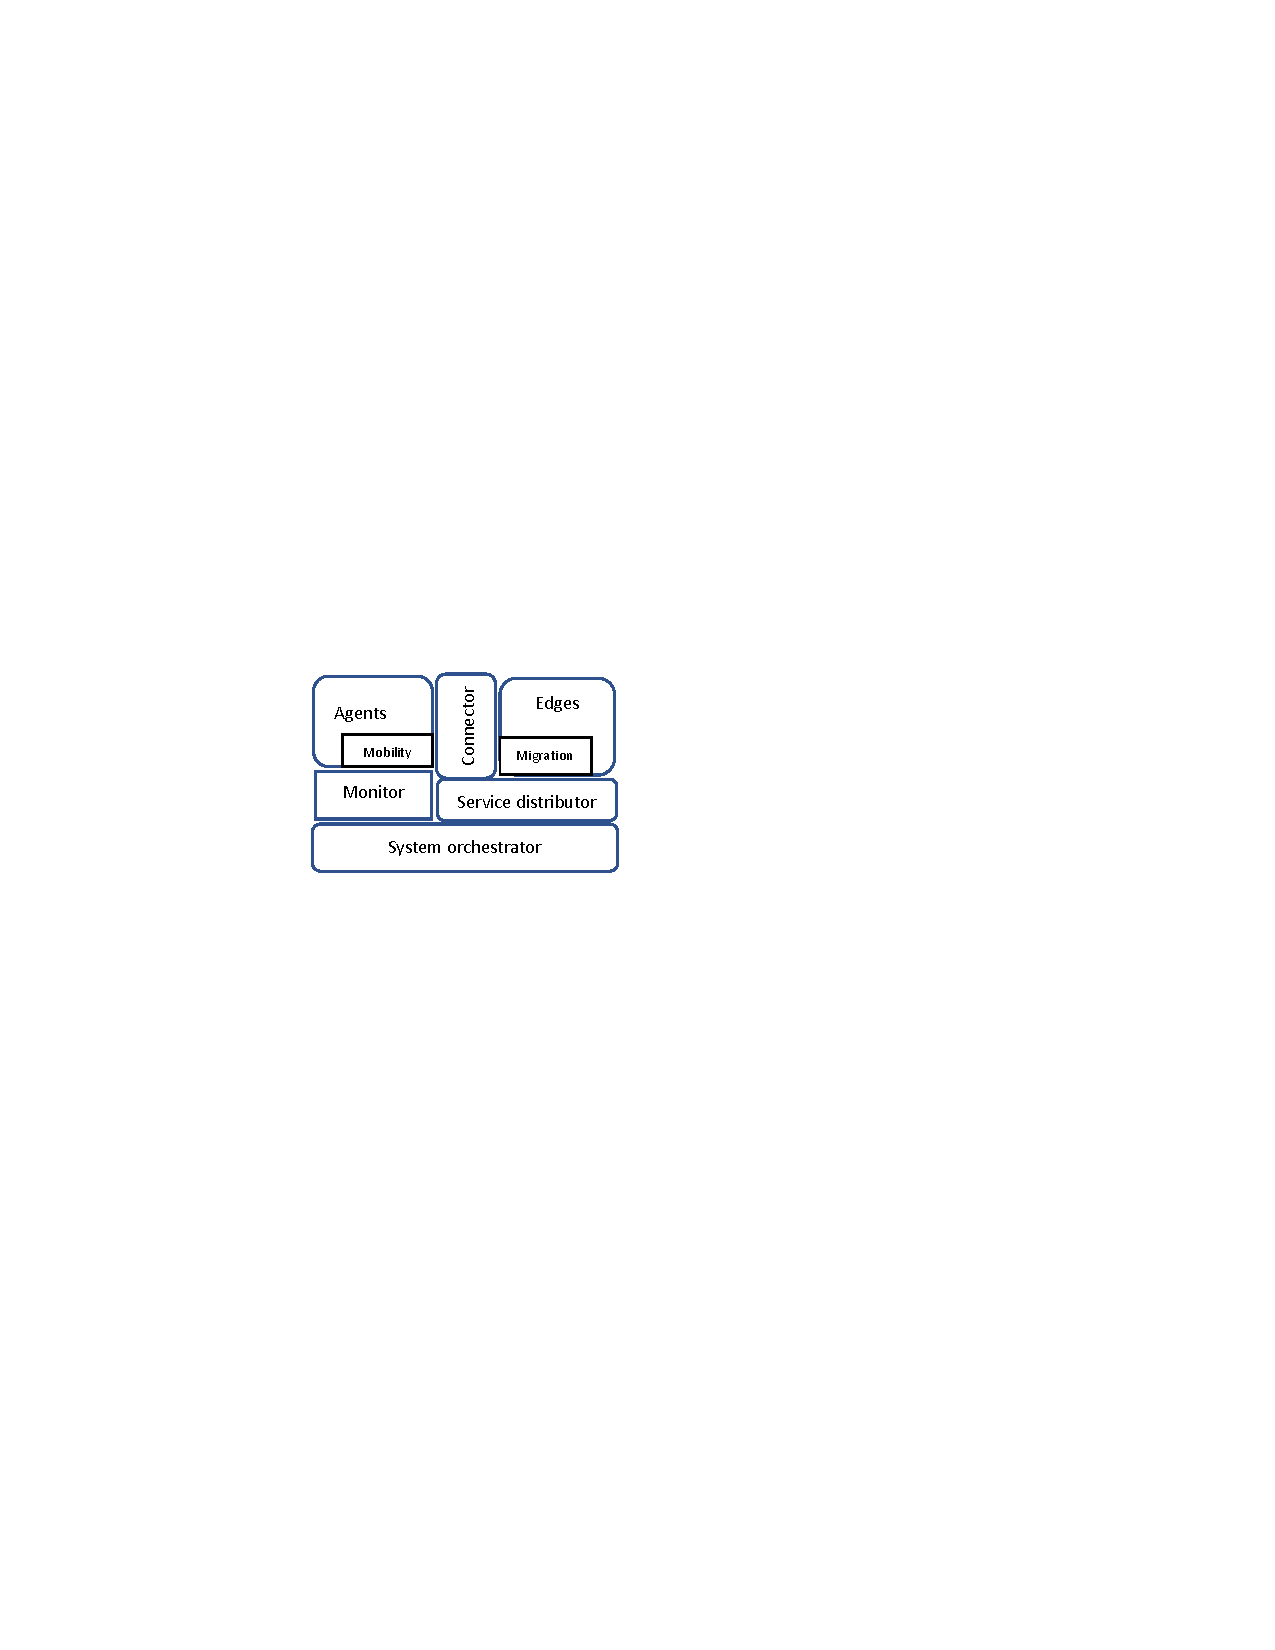
\includegraphics[clip, trim=3cm 13.0cm 9.5cm 11.2cm, width=\columnwidth]{figures/model5.pdf}
\caption{ATEDGEV2I testbed model}
\label{fig:model}
\end{figure}

\subsection{Agent}
\par An agent is an abstraction of a mobile entity such as vehicle or mobile device equipped with a set of sensors (e.g., GPS, camera), enabling the surrounding environment perception (e.g., position, speed, temperature) and a set of actuators (e.g., display, acceleration). Each agent has a mobility profile. This module's tasks consist of initiating/updating mobile node's position, creating/destroying communication's links, and managing mobility.
The mobility support is achieved through the use of the mobile nodes' positions regarding the fixed edge nodes and the city map to create and destroy communication links in runtime.
\subsection{Edge infrastructure}
\par The edge infrastructure offers a distributed limited storage and processing capabilities in the vicinity of the agents to cope with the Cloud issues in running V2I applications regarding real-time services ultra-low latency requirements. The "edges" refers to the combination of base stations (or access points) and edge servers close to the mobile radio network. An edge can be anything from well-provisioned and centralized servers to far-flung and lightly provisioned embedded devices. Edges are connected to the orchestrator by joining the orchestrator's Kubernetes cluster, and running a small program in the form of containers for connecting them to the connector and agents (i.e., network management).
\subsection{Connector} 
\par Cellular networks are characterized by a wide communication range, high speed data communication, which allows a base station to maintain connectivity with and serve a network agent (vehicle) as long as possible. The upcoming Generation cellular networks (5G and 6G) are the leading technologies that promise native mobile edge computing capabilities\cite{slawomir2017next} to grant a very high network capacity that guarantees high throughput/bandwidth for demanding V2I applications like Augmented reality on autonomous vehicles and other vehicular communication technologies\cite{cheriftestbed}. In our testbed, connector ,playing the role of communication network, is responsible for connecting different entities together and synchronising data pipelines. The communication of vehicles with a serving entity through a network is also managed with the connector.
\subsection{System orchestrator}
\par The management layer named orchestrator keeps an comprehensive view on available edge resources and running services. The Testbed API also runs on orchestrator and presents a web portal to developers which provides authenticated users access to ATEDGEV2I resources and APIs. The orchestrator has a small footprint that can be as light as a Raspberry Pi. In summary it is responsible for:
\begin{itemize}
\item Scaling up and down the available resources as required by the running applications. 
\item Allocating and releasing the storage, networking, and compute resources offered by the service distributor.
\item Storing application images for faster instantiation procedure when it is required.
\item Providing support for fault and performance monitoring by collecting data about resources and running applications
and transmitting them to the monitor module.
\end{itemize}

\subsection{Service distributor}
\par This module manages the task of selecting the appropriate host for the services requested by agents. For this purpose the distributor should take the service requirements, available resources, and agents' positions into consideration.

\subsection{Monitor}
\par Besides the web portal that provides utilization information for all connected nodes each experiment is provided a directory, shared among all containers in the experiment, which will persist after the experiment output. When an experiment concludes, the persistent directory will be available to the user through the web portal.
\section{Architecture/implementation}
\par ATEDGEV2I proposes an easy-to-use edge computing testbed system providing experimental environments for V2I application via APIs. We implemented an 8-node prototype of ATEDGEV2I at UoL comprising of one orchestrator node, one client host, one cloud server, and 6 edge nodes. In this section, we describe the architecture, implementation, and configuration of this prototype. 
\par The general architecture and the essential components of our proposed testbed are illustrated in Figure.\ref{fig:arch}. The testbed system provides services in the form of networked docker containers and client programs hosted on client host to testbed users. 
\begin{figure}[!htbp]
\centering
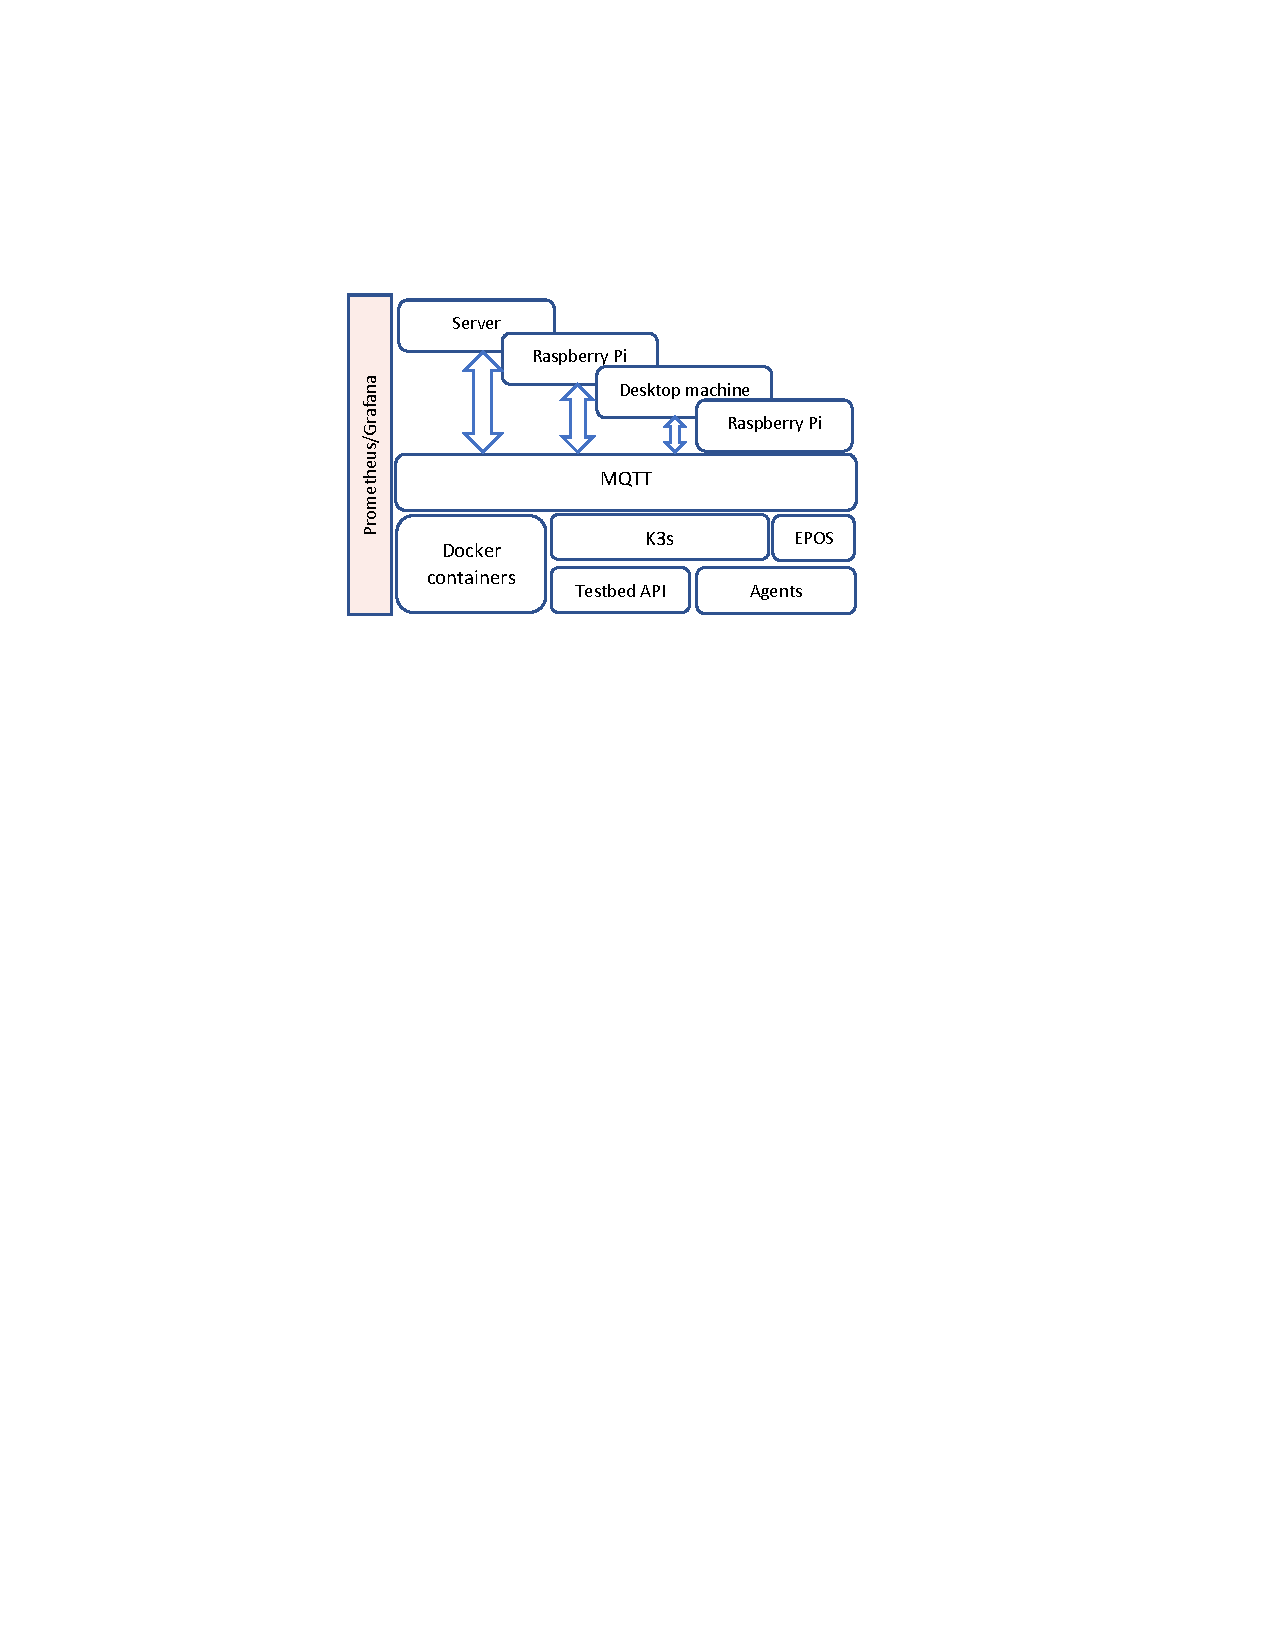
\includegraphics[clip, trim=4.7cm 17.5cm 5.9cm 5cm, width=\columnwidth]{figures/arch4.pdf}
\caption{Proposed test-bed architecture}
\label{fig:arch}
\end{figure}
%\fbox{
\subsection{Experimental testbed}
\par Table.\ref{tab:HW} summarizes the specifications of the hardware and software platform used in our experimental 
testbed. A router?? connects edge nodes to the access network via wired Ethernet??. 
We set up a server machine that runs Ubuntu?? to serve as the cloud. WLAN access point

\begin{table}[htbp]
\caption{Specification of hardware and software platform used in experimental testbed.}
\begin{center}
\begin{tabular}{|c|c|c|c|c|}
\hline
\textbf{Characteristic}&\multicolumn{4}{|c|}{\textbf{Device}} \\
\cline{2-5} 
\textbf{} & \textbf{\textit{Edge device}}& \textbf{\textit{Orchestrator}}& \textbf{\textit{Cloud server}}& \textbf{\textit{Client host}} \\
\hline
CPU& More table copy$^{\mathrm{a}}$& &  \\
\hline
RAM& More table copy$^{\mathrm{a}}$& &  \\
\hline
Disk& More table copy$^{\mathrm{a}}$& &  \\
\hline
OS& More table copy$^{\mathrm{a}}$& &  \\
\hline
\multicolumn{5}{l}{$^{\mathrm{a}}$Sample of a Table footnote.}
\end{tabular}
\label{tab:HW}
\end{center}
\end{table}

\subsection{ATEDGEV2I API}
\par ATEDGEV2I API is the core component of the testbed. It implements the required functions to create the edge environment. Users define experiments as (i) a set of edge resources along with their geographic location and resource specification, and (ii) a set of agents with their mobility profile and services requirements. The services are provided in the form of Docker containers and instantiated according to their resource requirements for allocations of RAM and CPU. Users provide ATEDGEV2I access to the service containers either through Dockerhub or a private docker repository. The testbed API interacts with orchestrator, i.e. Kubernetes, to instantiate the edge nodes from Raspberry Pies and then instantiate V2I application components from pre-created Docker container images. ATEDGEV2I containers are allocated and scheduled using a combination of the Kubernetes scheduler and the ATEDGEV2I service distributor described in next sections.
\par The testbed API implements an abstraction for edge nodes that are necessary to build a network environment. This abstraction allows the developer to apply resource models that define the available resources for each edge node, and interact with the real components. This also allows the management of a related set of edge server and edge access points as a single entity. 
\subsection{Raspberry Pi}
\par We have built ATEDGEV2I using Raspberry Pies, which their price is not high. Each Pi has a fixed position (coordinate) in a city that is the input provided by the developer. Migration controller module runs on edge nodes which guarantee the continuity of running services and handles the migration-related functions.
\subsection{Agent and Docker container}
\par Docker containers are preferable for a smooth transition of tested application programs to production environments.
In order to guarantees the security of internal containers and further simplifies users' work, ATEDGEV2I instantiates a container agent between a mobile end-device and internal containers. This container emulates a mobile device and makes its data transmission transparent. We also utilize docker containers to deploy users' application on Pies because of their characteristics: open source, light weight, fast startup and small resource consumption. 
\par The container agent receives testing data from end devices or other fog nodes. The testing data flow is produced by the testing app running on the end devices and sent to the container agent running on client host; then the container agent transfers the data to a corresponding docker service container. When a container running in an edge node wants to send data to a client, it should transfer the data to the container agent running on client, and then the local container agent will connect to the destination node and transfer the data to it, so the container agent is the bridge between end devices and testbed internal containers.
\subsubsection{Mobility}
\par Mobility monitor runs on mobile end devices. The Mobility monitor keeps updating the mobility profile of agent and the distance from itself to its current connected Pi; if it finds the distance is more than a threshold, it will send a connection (migration) request to another Pi with the lowest distance. Here, as shown in Figure.\ref{fig:mig} the threshold means the difference between the coverage range and the handover distance. At the same time the agent sends a notification to its current connected Pi to inform the node about the migration.
\par The developed mobility API can be used to implement different mobility models. A real-world map, in our tests Munich city map, could be imported to the SUMO traffic simulator\cite{behrisch2011sumo} to model an accurate mobility model that simulates vehicle movements. The mobility module interprets the source mobility database saved in .csv format.
Each .csv file represents the mobility profile of an agent (vehicle) in the form of a sequence of traversed points during the simulation. Each point includes: (i) position x and y on the map; (ii) speed in metres per second; (iii) the direction in radiants; and (iv) the simulation time in which these data is collected.

\subsection{K3s}
\par The testbed orchestrator, i.e. K3s master node, is the module interfacing with the testbed API and managing the edge resource allocation and releasing. Each of the Pies is a K3s worker node with additional modules for compatibility with the testbed. K3s is a light Kubernetes distribution which is faster to start up, and easier to auto-update and learn. It has a very small binary size and very low resource requirements that makes it suitable for edge environments and Pies.
K3s master node allows the orchestration, scaling, and management of a cluster of containers

\subsection{MQTT}
\par ATEDGEV2I leverages MQTT bi-directional messaging system as the connector of edges and agents. Its extremely lightweight publish/subscribe design makes this standard messaging protocol ideal for resource-constrained environments of Pies. 
In real scenario the network connects the edges and wireless base station nodes. The client host accesses its service container through the wireless base stations and the network. In our testbed deployment, as it is mentined already, edges are an abstraction of edge servers and their connected base station. In other word, the wireless base stations are wired network nodes whose their positions in the network correspond to wireless base stations in a mobile backhaul network. 
This imitated infrastructure is compatible with the edge computing infrastructure model in the 5G network proposed by ETSI\cite{etsi2018white}. As user plane functions in the 5G network infrastructure model  locate the edge nodes at any node in the edge computing testbed’s network.

\subsection{EPOS as Service distributor}
\par The service distributor makes decision on computation offloading and the placement of service containers that are waiting for resource allocation. When the decision is made, the containers are scheduled on their assigned edge nodes through K3s master node. The entities in ATEDGEV2I are decentralized; they are able to allocate resources of their environment independently. There exist two possibilities for making a computation offloading decision about where to offload (i.e., edge node or cloud server). The decision can be made by either a central coordinator based on the QoS requirements of mobile agents or independently the associated edge device itself. In our experiment, we apply the first offloading approach to help reduce the complexity, however, the second approach is also applicable.
\par For a request of a service Docker container by the testbed user, ATEDGEV2I automatically determines the Pi that satisfies the service requirements and configures the Docker container on that Pi. ATEDGEV2I utilizes EPOS\cite{pournaras2018decentralized}, a fully decentralized networked system designed for participatory multi-objective optimization. It performs collective decision-making among edges that autonomously generate a set of placement maps from which they make a choice. The edges get informed of the placement decision through their shared volumes with EPOS.

\section{Testbed workflow}
\par Although the ATEDGEV2I system takes away the configurability of a K3s system due to using the virtual
region-based interface, it is enough for testbed users who are IoT application developers. The main lost configurability is direct server selection to place Docker containers and network policy setting to control communication among
Docker containers. However, IoT application developers do not need this configurability because, typically in IoT applications, communication occurs between clients and servers nearby proximity while the proposed testbed system supports that communication pattern.
In terms of human resources for testbed system management, the proposed testbed system has extra maintenance
costs in addition to that of the k8s system because a system administrator needs to maintain both the k8s and the testbed
manager. However, both systems keep running without human operations. Thus, in normal operations, the human resources for maintaining the proposed testbed system are almost the same as that of K3s.

\begin{figure*}
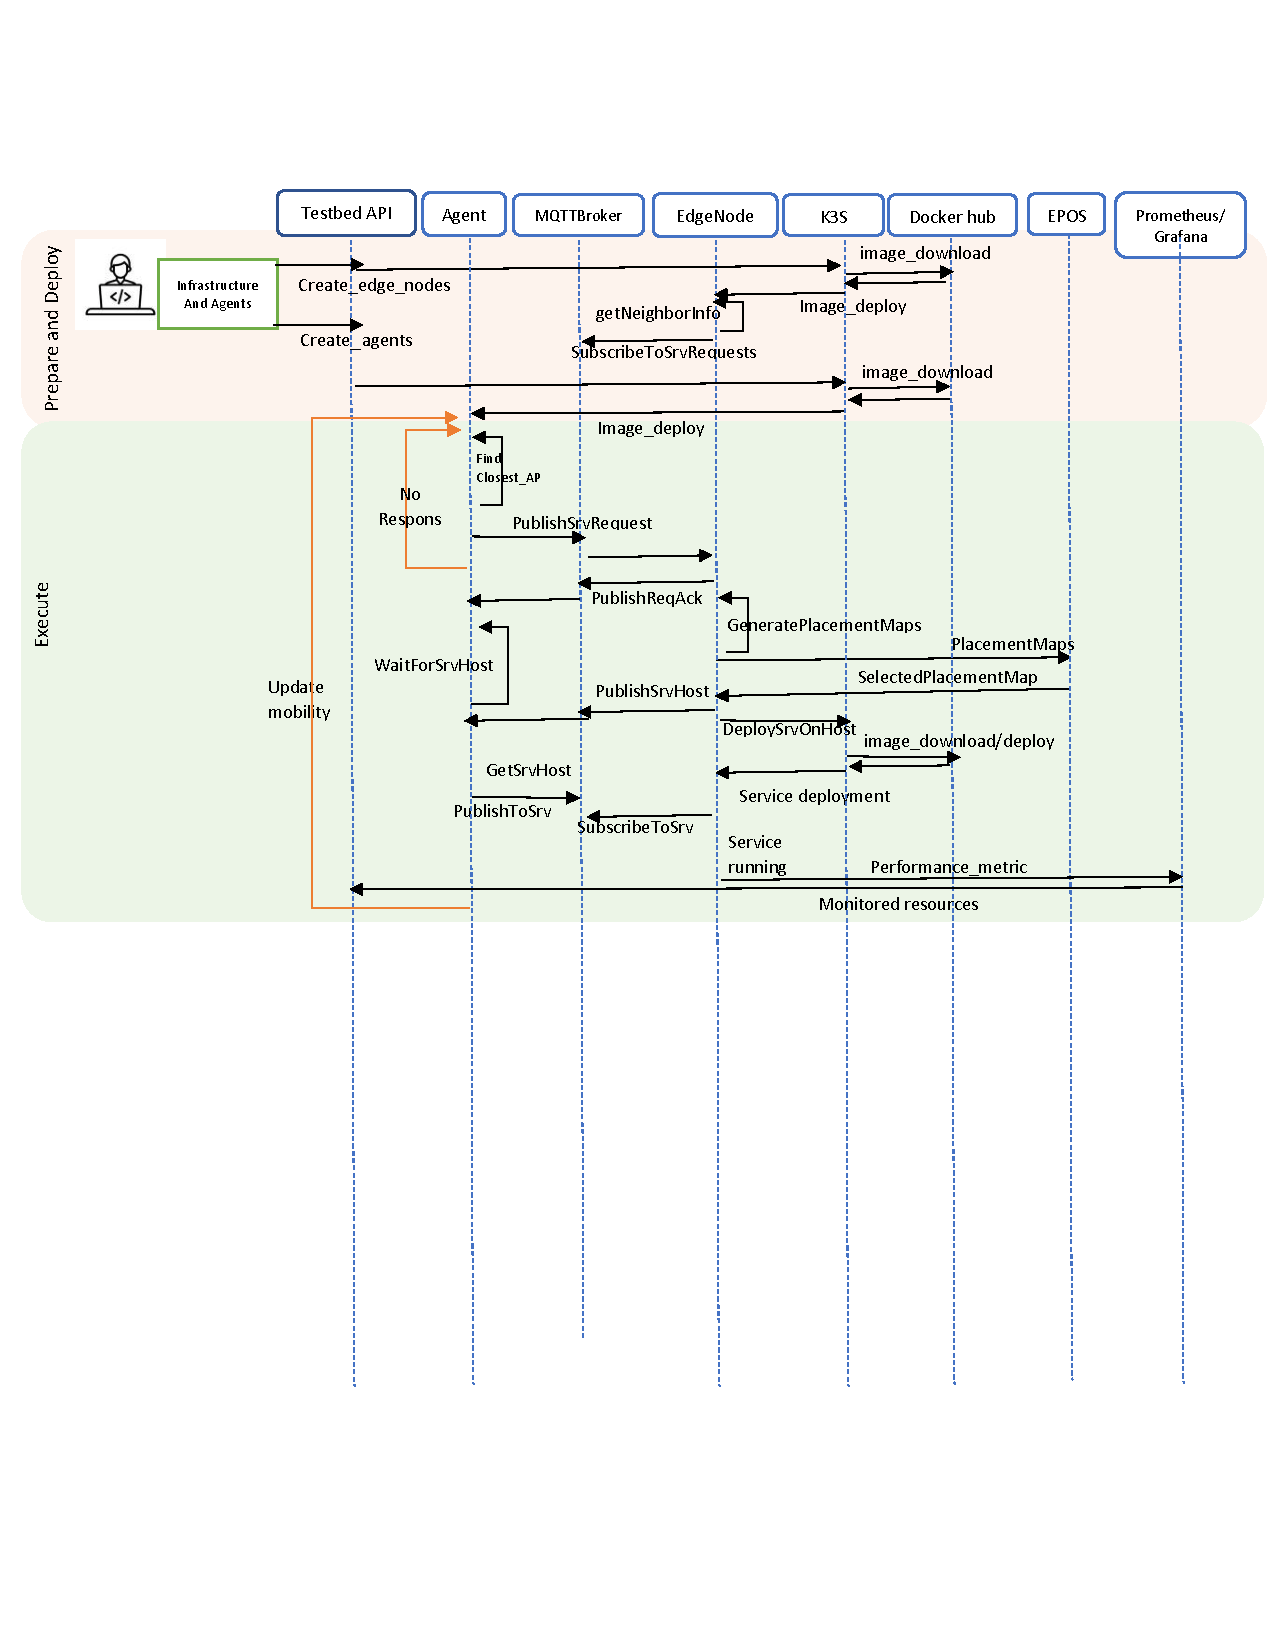
\includegraphics[clip, trim=0.2cm 12.3cm 0.3cm 3.2cm, width=\textwidth]{figures/workflow-4.pdf}
\caption{V2I application workflow}
\label{fig:workflow}
\end{figure*}

\section{Applications}
\par The workflow of creating and evaluating atypical V2I application using our testbed is demonstrated in the Fig.\ref{fig:workflow}.


\subsection{Services????}
\par Deploying Services in the form of Docker instances offers a virtualized isolated environment for service execution at each host. The use of virtual interfaces and virtual links allows different nodes and instances to communicate easily.
\begin{figure}[!htbp]
\centering
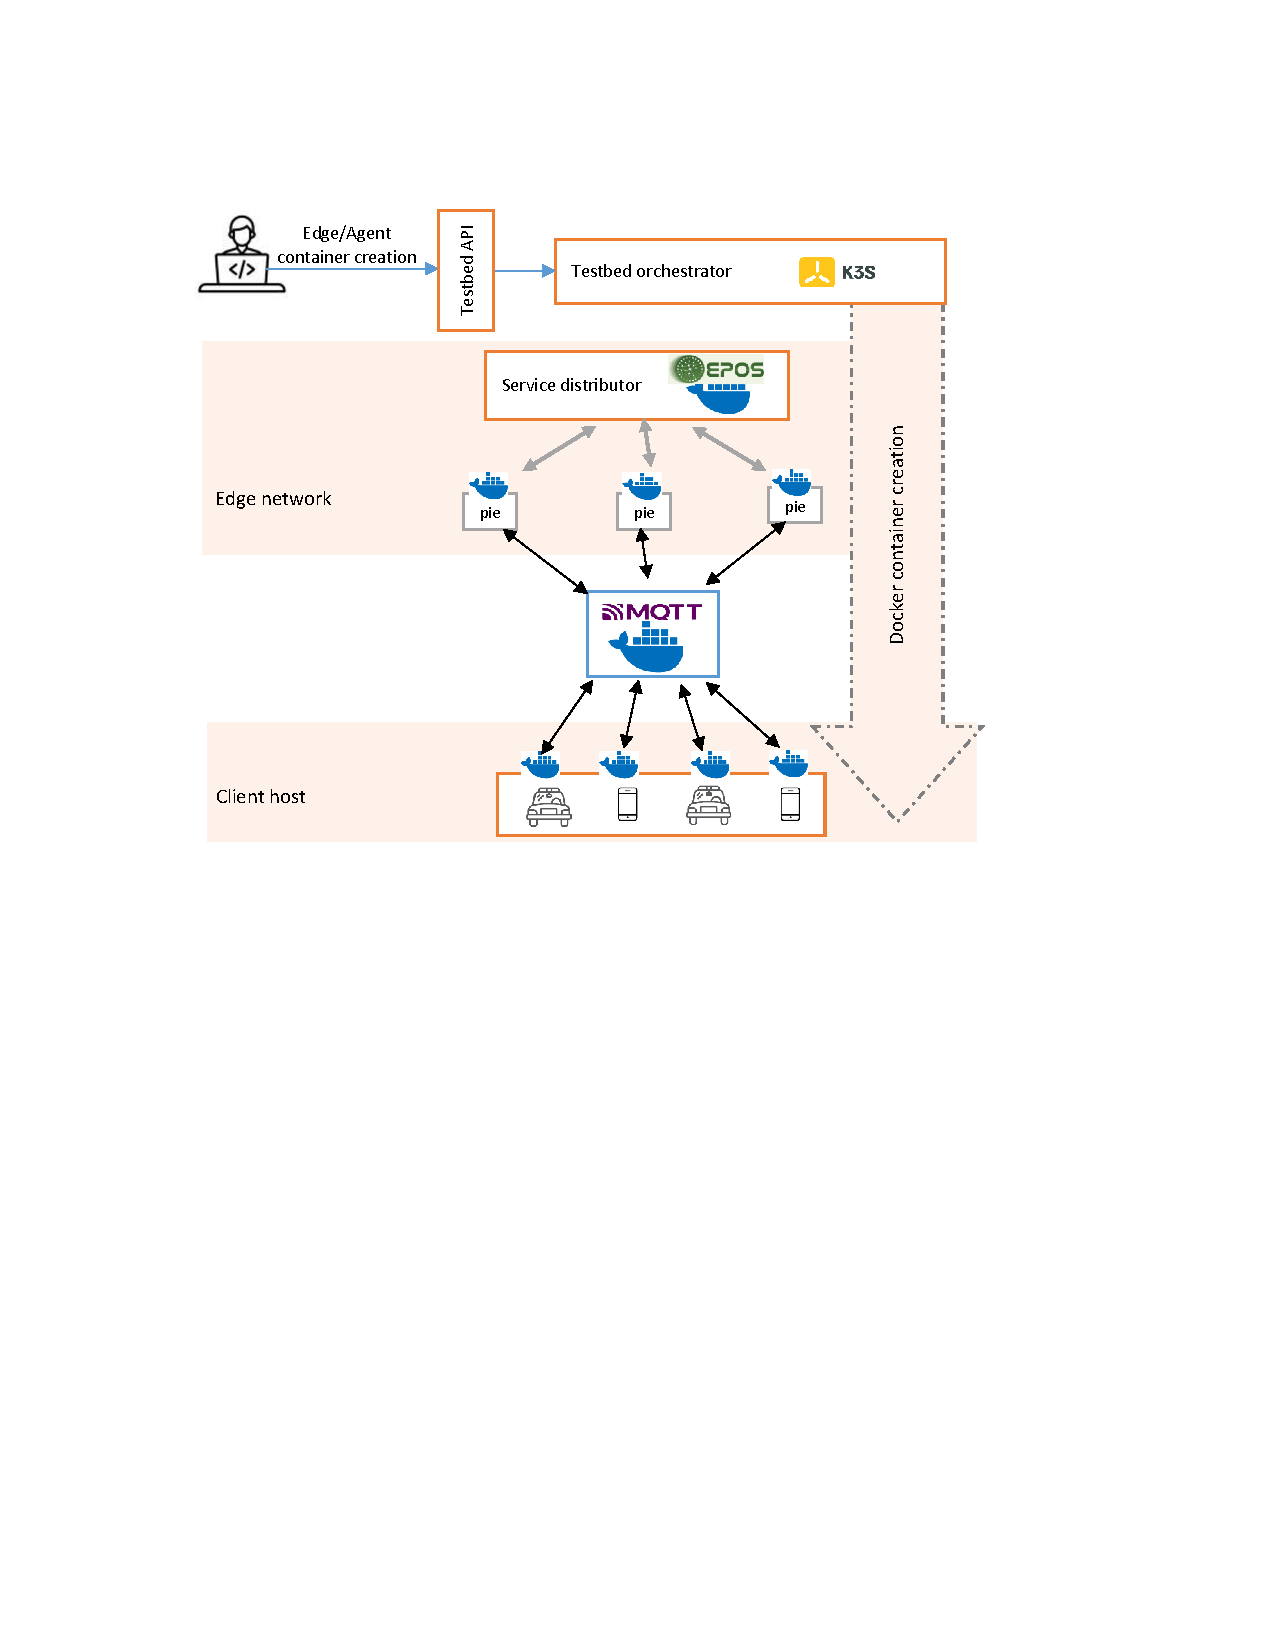
\includegraphics[clip, trim=3.3cm 13.7cm 4.5cm 3.5cm, width=\columnwidth]{figures/app1.pdf}
\caption{Vehicles traffic monitoring service architecture}
\label{fig:imp}
\end{figure}
Assuming an experimental user develops an edge application to count, in real-time, pedestrian
volume passing a road, and he wants to test the function and performance of each part of the application.
We suppose that the application consists of three modules: a data aggregate module 
running on the cloud node, a pedestrian flow collection module running on several fog nodes and a 
client app running on users' end devices. As the end device is moved, the client app will connect to 
the pedestrian flow collection application running on the fog node; each fog node periodically sends 
the statistical data to the data aggregate module running on the cloud node. Suppose that the user 
Figure 2. Component interactions in each stage of an experiment.
Assuming an experimental user develops an edge application to count, in real-time, pedestrian
volume passing a road, and he wants to test the function and performance of each part of the application.
We suppose that the application consists of three modules: a data aggregate module running on the
cloud node, a pedestrian flow collection module running on several fog nodes and a client app running
on users’ end devices. As the end device is moved, the client app will connect to the pedestrian flow
Sensors 2020, 20, 1900 6 of 15
collection application running on the fog node; each fog node periodically sends the statistical data to
the data aggregate module running on the cloud node. Suppose that the user has generated two docker
images, which include the data aggregate module and data collection module respectively, and stored
them on the Doker Hub, which is the world’s largest library for docker container images. The two
images will run on a cloud node and several fog nodes, respectively, later. The user wants to utilize
mobile crowdsourcing devices to continuously count the pedestrian volume of a road during a period
of time, so he publishes the purpose and demand of the experiment to the piFogBedII platform in
advance, which will push the experiment information to users who subscribe to that type of experiment.
All end devices participating in the experiment must be installed the endworker, registered on the
piFogBedII. Then, the user carries out his experiment according to the following four stages

Application Layer Overview: From an edge application perspective, three use case scenarios are considered for computation offloading in the following.

Non-Offloading Scenario: In this scenario, the end device executes the computation task locally. In compute-intensive applications such as real-time object detection applications the view 
controller on the edge/mobile device captures image frames from the live camera and sends the captured frames to the object detection client module for computation. The object detection client module executes the computation task and then returns the result. 
Access Edge Cloud Offloading Scenario: In this scenario, the edge/mobile device establishes a 
reliable communication via transmission control protocol (TCP) with the access edge cloud, where 
an instance of a multithreaded face detection 
server module is running on top of OpenStack++. 
Once the connection is established successfully, 
the edge/mobile device offloads the computation 
task onto the access edge cloud. Upon receiving a request, the face detection server module 
executes the offloaded computation task using 
the OpenCV library. Afterward, the server compresses the result frames and sends them back 
to the face detection client module upon completion. Finally, the view controller receives the 
results from the face detection client module and 
visualizes the result.
Metro Edge Cloud Offloading Scenario: This 
scenario works in a similar fashion as the access 
edge cloud scenario. More precisely, the face 
detection client module establishes a connection with the metro edge cloud, which runs an 
instance of the multithreaded server module on 
top of OpenStack. After receiving the offloaded 
task, the server module executes the computation. The server module then compresses the 
result frames and sends them back to the edge 
device upon completion.


\section{Evaluation}


\subsection{Threats to validity}


\subsection{Conclusion}
\par While it is very important to test functions and performances of various applications before they are deployed to
the production environment, current evaluations are more based on simulation tools. As the fidelity of the experimental results is a problem for most of simulation tools, in this paper we present ATEDGEV2I testbed...
To evaluate the performance of our developed testbed, we designed a resource management scheme, developed an application, and performed computation offloading onto edge nodes.

%\section*{References}

\bibliographystyle{plain}
\bibliography{mybib}

\end{document}
